\section{Understandability Study (RQ2)}
\label{sec:understandability}
The overall idea of this study  is to present  programmers with one of several representations of semantically equivalent regexes and ask comprehension questions. By comparing the understandability of semantically equivalent regexes that have different representations, we aim to understand which representations  are more desirable and which are more smelly.
This study was  implemented on Amazon's Mechanical Turk with 180 participants.  Each regex pattern was evaluated by 30 participants.
The patterns used were designed to belong to various representations in Figure~\ref{fig:refactoringTree}.

\begin{figure}[tb]
\centering
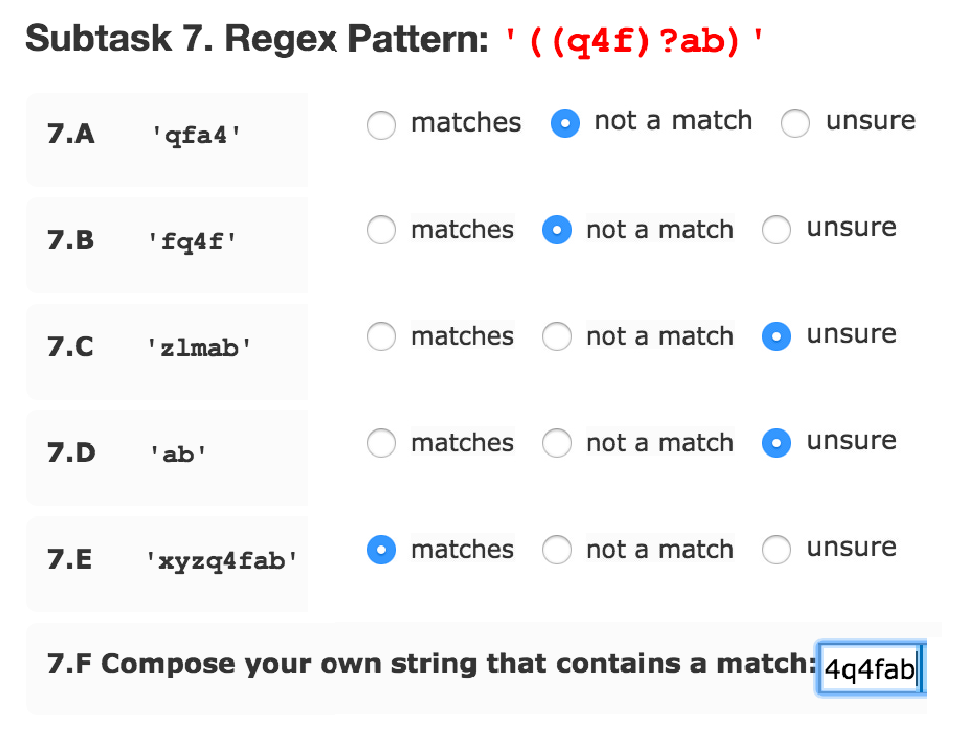
\includegraphics[width=0.8\columnwidth]{nontex/illustrations/exampleQuestion.eps}
\vspace{-12pt}
\caption{Example of one HIT Question}
\vspace{-6pt}
\label{fig:exampleQuestion}
\end{figure}

\begin{table}
\caption{Matching metric example \label{matchingmetric}}
\begin{center}
\begin{small}
\begin{tabular} {cl | c c c c c}
\textbf{String} & \verb!`RR*'! & \textbf{Oracle} & \textbf{P1} & \textbf{P2} & \textbf{P3}& \textbf{P4}\\ \hline
1 & ``ARROW"    & \checkmark    & \checkmark    & \checkmark    & \checkmark    & \checkmark \\
2 & ``qRs"      & \checkmark    & \checkmark    & \xmark        & \xmark        & ?\\
3 & ``R0R"      & \checkmark    & \checkmark    & \checkmark    & ?             & -\\
4 & ``qrs"      & \xmark        & \checkmark    & \xmark        & \checkmark    & -\\
5 & ``98"       & \xmark        & \xmark        & \xmark        & \xmark        & -\\
\hline
  & Score       & 1.00          & 0.80          & 0.80          & 0.50          & 1.00\\
\\
\multicolumn{7}{l}{\checkmark = match, \xmark = not a match, ? = unsure, -- = left blank}\\
\end{tabular}
\end{small}
\end{center}
\end{table}


\subsection{Metrics}
\label{sec:understadningmetric}
We measure the understandability of regexes using two complementary metrics, \emph{matching} and \emph{compostition}.

\textbf{Matching:}
Given a pattern and a set of strings, a participant determines which strings will be matched by the pattern. There are four possible responses for each string, \emph{matches}, \emph{not a match}, \emph{unsure}, or blank. An example from our study is shown in Figure~\ref{fig:exampleQuestion}.

The percentage of correct responses, disregarding blanks and unsure responses, is the matching score.
For example, consider regex pattern \verb!`RR*'! and five strings shown in Table~\ref{matchingmetric}, and the responses from four participants in the \emph{P1}, \emph{P2}, \emph{P3} and \emph{P4} columns.
The oracle has the first three strings matching since they each contain at least one \verb!R! character. \emph{P1} answers correctly for the first three strings but incorrectly thinks the fourth string matches, so the matching score is $4/5 = 0.80$. \emph{P2} incorrectly thinks that the second string is not a match, so they also score $4/5 = 0.80$.  \emph{P3} marks `unsure' for the third string and so the total number of attempted matching questions is 4 instead of 5. \emph{P3} is incorrect about the second and fourth string, so they score $2/4 = 0.50$.  For \emph{P4}, we only have data for the first and second strings, since the other three are blank.  \emph{P4} marks `unsure' for the second matching question so only one matching question has been attempted, and it was answered correctly so the matching score is $1/1 = 1.00$.

Blanks were incorporated into the metric because questions were occasionally left blank in the study. Unsure responses were provided as an option so not to bias the  results when participants were honestly unsure of the answer. These situations did not occur very frequently. Only 1.1\% of the responses were left blank and only 3.8\% of the responses were marked as unsure.  We refer to a response with all blank or unsure responses as an `NA'. Out of 1800 questions, 1.8\%(32) were NA's (never more than 4 out of 30 per pattern).

\textbf{Composition:}
Given a pattern, a participant composes a string they think it matches. If the participant is accurate and the string indeed is matched by the pattern, then a composition score of 1 is assigned, otherwise 0.  For example, given the pattern \verb!`(q4fab|ab)'! from our study, the string, ``xyzq4fab" matches  and would get a score of 1, and the string, ``acb" does not match and would get a score of 0.

To determine a match, each pattern was compiled using the \emph{java.util.regex} library. A \emph{java.util.regex.Matcher} \verb!m! object was created for each composed string using the compiled pattern.  If \verb!m.find()! returned true, then that composed string was given a score of 1, otherwise it was given a score of 0.

\subsection{Design}
This study was implemented on the Amazon's Mechanical Turk (MTurk),  a crowdsourcing platform in which requesters can create human intelligence tasks (HITs) for completion by workers. Each HIT is designed to be completed in a fixed amount of time and workers are compensated with money if their work is satisfactory. Requesters can screen workers by requiring each to complete a qualification test prior to completing any HITs.

\subsubsection{Worker Qualification}
Workers qualified to participate in the study by answering questions regarding some basics of regex knowledge. These questions were multiple-choice and asked the worker to describe what the following patterns mean: \verb!`a+'!, \verb!`(r|z)'!, \verb!`\d'!, \verb!`q*'!, and \verb!`[p-s]'!. To pass the qualification, workers had to answer four of the five questions correctly.

\subsubsection{Tasks}
Using the patterns in the corpus as a guide, we created 60 regex patterns that were grouped into 26 semantic equivalence groups.
These semantic groups were focused on exploring edges in the equivalence classes. In this way, we can draw conclusions about transformations between representations since the regexes evaluated were semantically equivalent.

For example, a  group with regexes \verb!`([0-9]+)\.([0-9]+)'! and  \verb!`(\d+)\.(\d+)'! is intended to evaluate the edge between C1 and C4.
There were 18 groups with two regexes that target various edges in the equivalence classes.
The other eight semantic groups had three regexes each.
For example, a semantic group with regexes \verb!`((q4f){0,1}ab)'!, \verb!`((q4f)?ab)'!, and \verb!`(q4fab|ab)'! is intended to explore the edges among D1, D2, and D3.

\todoNow{Smooth this section with description included}
Using the patterns in the corpus as a guide, we created six metagroups containing three pairs of patterns focusing on:
\begin{itemize}
\item S1 vs S2
\item the digit default character class vs C1
\item the word default character class vs C1
\item negated digits and words vs C3, whitespace vs C2
\item additional vs kleene repetition
\item wrapping vs escaping literal characters
\end{itemize}
and four metagroups containing two triplets of patterns focusing on
\begin{itemize}
\item octal vs hex vs literal
\item D1 vs D2 vs D3
\item C1 vs C2 vs C5
\item octal vs literal and C2 vs C5
\end{itemize}

Each of these 10 metagroups contains 6 strings, resulting in a total of 60 regex patterns.  These patterns are logically partitioned into 26 semantic equivalence groups (18 from pairs, 8 from triples).

For each of the 26 groups of patterns, we created five strings, where at least one matched and at least one did not match. These strings were used to compute the matching metric.

Once all the patterns and matching strings were collected, we created tasks for the MTurk participants as follows:
randomly select a pattern from each of the 10 metagroups. Randomize the order of these 10 patterns, as well as the order of the matching strings for each pattern. After adding a question asking the participant to compose a string that each pattern matches, this creates one task on MTurk.   This process was completed until each of the 60 regexes appeared in 30 HITs, resulting in a total of 180 total unique HITs.
An example of a single regex pattern, the five matching strings and the space for composing a string is shown in Figure~\ref{fig:exampleQuestion}.

\subsubsection{Implementation}
Workers were paid \$3.00 for successfully completing a HIT, and were only allowed to complete  one HIT.  The average completion time for accepted HITs was 682 seconds (11 mins, 22 secs).
A total of 55 HITs were rejected, and  of those, 48 were rushed through by one person leaving many answers blank, 4 other HITs were also rejected because a worker had submitted more than one HIT, one was rejected for not answering composition sections, and one was rejected because it was missing data for 3 questions.  Rejected HITs were returned to MTurk to be completed by others.

\begin{figure}[tp]
\begin{small}
\fbox{\parbox{\columnwidth}{
\begin{enumerate}
\item
\begin{tabular} {lrr}
\textbf{What is your gender?} & \textbf{n} & \textbf{\%}\\ \hline
Male & 149 & 83\%\\
Female & 27& 15\%\\
Prefer not to say & 4& 2\%
\end{tabular}
\item \textbf{What is your age?} \\
$\mu = 31$, $\sigma = 9.3$

\item

\begin{tabular} {l |rr}
\textbf{Education Level?} & \textbf{n} & \textbf{\%}\\ \hline
High School & 5 & 3\%\\
Some college, no degree & 46 & 26\%\\
Associates degree & 14 & 8\%\\
Bachelors degree & 78 & 43\%\\
Graduate degree & 37 & 21\%\\
\end{tabular}
\item
\begin{tabular} {lrr}
\textbf{Familiarity with regexes?} & \textbf{n} & \textbf{\%}\\ \hline
Not familiar at all & 5 & 3\%\\
Somewhat not familiar & 16 & 9\%\\
Not sure & 2 & 1\%\\
Somewhat familiar & 121 & 67\%\\
Very familiar & 36 & 20\%\\
\end{tabular}
\item \textbf{How many regexes do you compose each year?} \\
$\mu = 67$, $\sigma = 173$
\item \textbf{How many regexes (not written by you) do you read each year?} \\
$\mu = 116$, $\sigma = 275$
\end{enumerate}
}}
\caption{Participant Profiles, $n=180$ \todoLast{can remove this for space} \label{participantprofile}}
\end{small}
\end{figure}

\subsection{Participants}

In total, there were 180 participants in the study.
A majority were male (83\%) with an average age of 31. Most had
at least an Associates degree (72\%) and most were at least somewhat familiar with regexes prior to the study (87\%). On average,
participants compose 67 regexes per year with a range of 0 to 1000.
Participants read more regexes than they write with an average of 116 and a range from 0 to 2000.
Figure~\ref{participantprofile} summarizes the self-reported participant characteristics from the qualification survey.

\begin{table*}\begin{small}\begin{center}\caption{Averaged Info About Edges (sorted by lowest of either p-value)}\label{table:testedEdgesTable}\begin{tabular}
{llccccccc}
Index & Nodes & Pairs & Match1 & Match2 & $H_0^{match} $ & Compose1 & Compose2 &  $H_0^{comp}$ \bigstrut \\
\toprule[0.16em]
E1 & T1 -- T4 & 2 & 0.80 & 0.60 & 0.001 & 0.87 & 0.37 & \textbf{$<$0.001}\\
E2 & D2 -- D3 & 2 & 0.78 & 0.87 & \textbf{0.011} & 0.88 & 0.97 & 0.085\\
E3 & L2 -- L3 & 3 & 0.86 & 0.91 & \textbf{0.032} & 0.91 & 0.98 & 0.052\\
\midrule[0.16em]
E4 & C2 -- C5 & 4 & 0.85 & 0.86 & 0.602 & 0.88 & 0.95 & {0.063}\\
E5 & C2 -- C4 & 1 & 0.83 & 0.92 & {0.075} & 0.60 & 0.67 & 0.601\\

E6 & D1 -- D2 & 2 & 0.84 & 0.78 & 0.120 & 0.93 & 0.88 & 0.347\\
E7 & C1 -- C2 & 2 & 0.94 & 0.90 & 0.121 & 0.93 & 0.90 & 0.514\\
E8 & T2 -- T4 & 2 & 0.84 & 0.81 & 0.498 & 0.65 & 0.52 & 0.141\\
E9 & C1 -- C5 & 2 & 0.94 & 0.90 & 0.287 & 0.93 & 0.93 & 1.000\\
E10 & T1 -- T3 & 3 & 0.88 & 0.86 & 0.320 & 0.72 & 0.76 & 0.613\\
E11 & D1 -- D3 & 2 & 0.84 & 0.87 & 0.349 & 0.93 & 0.97 & 0.408\\
E12 & C1 -- C4 & 6 & 0.87 & 0.84 & 0.352 & 0.86 & 0.83 & 0.465\\
E13 & C3 -- C4 & 2 & 0.61 & 0.67 & 0.593 & 0.75 & 0.82 & 0.379\\
E14 & S1 -- S2 & 3 & 0.85 & 0.86 & 0.776 & 0.88 & 0.90 & 0.638\\
\bottomrule[0.13em]\end{tabular}\end{center}\end{small}\end{table*}


\todoMid{in study section present choices about pairwise vs random selection for nodes.}

\subsection{Analysis}
For each of the 180 HITs, we computed a matching and composition score for each of the 10 regexes, using the metrics described in Section~\ref{sec:understadningmetric}. This allowed us to compute and then average 26-30 values for each metric  for each of the 60 regexes (fewer than 30 values were used if all the responses in a matching question were unsure or a combination of blanks and unsure).

Each regex was a member of one of 26 groupings of equivalent regexes.
These groupings allow pairwise comparisons of the metrics values to determine which representation of the regex was most understandable and the direction of a refactoring for understandability.
Among all the groups, we performed 42 pairwise comparisons of the matching and composition scores  (i.e., one comparison for each group of size two and three comparisons within each group of size three).
For example, one group had regexes, \verb!RR*! and \verb!R+!, which  represent a transformation between L2 and L3. The former had an average matching of 86\% and the latter had an average matching of 92\%. The average composition score for the former was 97\% and 100\% for the latter. Thus, the community found \verb!R+! from L3 more understandable.
There were two other pairwise comparisons performed between the L2 and L3 group, using regexes pair \verb!zaa*! and \verb!za+'!, and regexes pair \verb!\..*! and \verb!\.+'!.
Considering all three of these regex pairs, the overall matching average for the regexes belonging to L2 was 0.86 and 0.91 for L3.
The overall composition score for L2 was 0.91 and 0.98 for L3. Thus, the community found L3 to be more understandable than L2, from the perspective of both understandability metrics, suggesting a refactoring from L2 to L3.

This information is presented in summary in Table~\ref{table:testedEdgesTable}, with this specific example appearing in the E3 row. The \emph{Index} column enumerates all the pairwise comparisons evaluated in this experiment, \emph{Representations} lists the two representations, \emph{Pairs} shows how many comparisons were performed, \emph{Match1} gives the overall matching score for the first representation listed, \emph{Match2} gives the overall matching score for the second representation listed, and $H_0: \mu_{match1} = \mu_{match2}$ uses the Mann-Whitney test of means to compare the matching scores, and presents the p-values. The last three columns list the average composition scores for the representations and the p-value, also using the Mann-Whitney test of means.

\todoNow{smooth the explanation of comparisons and strings}
60 strings
42 comparisons
18@2, 8@3

M6R1 ? group 3, 3 comparisons
- 1 comparisons
- 0 strings

M3R0 ? group 3, 3 comparisons
- 1 comparisons
- 0 strings

M3R1 ? group 3, 3 comparisons
- 2 comparisons
- 1 string

M3R0 ? group 3, 3 comparisons
- 2 comparisons
- 1 string

58 strings
36 comparisons

Although we had 42 pairwise comparisons,  we had to drop six comparisons  due to a design flaw since the patterns performed transformations from multiple equivalence classes. For example, pattern \verb!([\072\073])! is in C2 and T4, and was grouped with pattern \verb!(:|;)! in C5, T1, so it was not clear if any differences in understandability were due to the transformation between C2 and C5, or T4 and T1. However, the third member of the group, \verb!([:;])!, could be compared with both, since it is a member of T1 and C2, so comparing it to \verb!([\072\073])! evaluates the transformation between T1 and T4, and comparing to \verb!(:|;)! evaluates the transformation between C2 and C5. The end result is 36 pairwise comparisons across 14 edges from Figure~\ref{fig:refactoringTree}.

\subsection{Results}
Table~\ref{table:testedEdgesTable} presents the results of the understandability analysis. A horizontal line separates the first three edges from the bottom 11. In E1 through E3, there is a statistically significant difference between the representations for at least one of the metrics considering $\alpha = 0.05$.  These represent the strongest evidence for suggesting the directions of refactoring based on the understandability metrics we defined. Specifically, $\overrightarrow{T4 T1}$, $\overrightarrow{D2 D3}$, and $\overrightarrow{L2 L3}$
are likely to improve understandability.

We note here that participants were able to select \emph{unsure} when they were not sure if a string would be matched by a pattern (Figure~\ref{fig:exampleQuestion}). From a comprehension perspective, this indicates some level of confusion and is worth exploring.

\begin{table*}
\centering
\caption{Average Unsure Responses Per Pattern By Node (fewer unsures are lower)}\label{table:unsureResults}
\begin{tabular}{ccc}
Node & Number of Patterns & Unsure Responses Per Pattern \\
T4 &  4 & 8.5  \\
T2 &  2 & 5.5  \\
T3 &  3 & 2.7  \\
T1 &  3 & 2.7  \\
D2 &  2 & 2.5  \\
C3 &  2 & 2   \\
C5 &  4 & 2   \\
D1 &  2 & 2   \\
C4 &  9 & 1.9  \\
S1 &  3 & 1.7  \\
S2 &  3 & 1.7  \\
L2 &  3 & 1.3  \\
C1 &  8 & 1  \\
C2 &  5 & 1  \\
D3 &  2 & 1  \\
L3 &  3 &0.7  \\
\end{tabular}
\end{table*}


For each pattern, we counted the number of responses containing at least one unsure, representing confusion.
We then grouped the patterns into their representation nodes and computed an average of unsures per pattern.
A higher number may indicate difficulty in comprehending a pattern from that node.
Overall, the highest number of unsure responses came from T4 and T2, which present octal and hex representations of characters. The least number of unsure responses were in L3 and D3, which are both shown to be understandable by looking at E2 and E3 in Table~\ref{table:testedEdgesTable}.
These nodes and their average number of unsure responses are organized by quartile in Table~\ref{table:unsureResults}.
These results also corroborate the refactorings suggested by the understandability analysis for the LIT group (i.e., $\overrightarrow{T4 T1}$), the DBB group (i.e.,  $\overrightarrow{D2 D3}$), and the LWB group (i.e., $\overrightarrow{L2 L3}$) because the more understandable node has the least unsures of its group.
The findings for D3 and D2 are contradictory, however, as  and further study is needed, and the number of unsures may be too small to indicate anything, except for T2 and T4.  The one pattern from T4 that had the most unsures of any pattern (i.e., 10 out of 30) was \verb!`xyz[\0133-\0140]'!, so this may have been the least understandable pattern that we tested.
\todoNow{Smooth over this unsure counts business}
